\documentclass[a4paper]{article}

\usepackage[english]{babel}
\usepackage[utf8x]{inputenc}
\usepackage{amsmath}
\usepackage{amssymb}
\usepackage{float}
\usepackage{graphicx}
\usepackage[colorinlistoftodos]{todonotes}
\usepackage[authoryear]{natbib}
\usepackage{hyperref}
\usepackage{authblk}
\usepackage[margin=1in]{geometry}
\usepackage{pgfplots}
\usepackage[T1]{fontenc}
\usepackage{parskip}
\usepackage{media9}

\pgfplotsset{compat=1.12}



\title{Bipedal Walker in OpenAI gym with Deep Deterministic Policy Gradients Algorithm}
\author{Khan Saad Bin Hasan, Arpit Varshney}
\date{\today} % You can write in any date within the brackets.

\begin{document}

\maketitle

\begin{abstract}
With the advent of Humanoid Robots and the advances in Robot assisted locomotion, there is a great need for robots that can learn to walk in complex environments. Hand Engineered approaches might work in constrained environments but learning based approaches may prove to be superior owing to their greater generalization. The goal of this work is to teach a bipedal robot to walk in a simulated environment.
\end{abstract}

\section*{Introduction}

Humanoid robots may prove to be superior to wheeled robots in certain circumstances owing to their high maneuverability and to work in similar environments as humans. Moreover, this can also help people with disabilities and help them move. As a result, bipedal locomotion is attracting more and more attention throughout the years. [\cite{song2017recurrent:2017}]

Most bipedal walking control are achieved using deterministic and analytic engineering approaches. Reinforcement learning can also be applied to model-free learning for bipedal walking in robots. This has been attempted in various action policy learning algorithms based on Markov Decision Process [\cite{song2017recurrent:2017}]

OpenAI Gym is a toolkit for reinforcement learning research. It includes a growing collection of benchmark problems that expose a common interface, and a website where people can share their results and compare the performance of algorithms. [\cite{brockman2016openai:2016}]

Bipedal robot is a simple 4-joints walker robot environment present in openAI gym with a normal version, with slightly uneven terrain and a Hardcore version with ladders, stumps, pitfalls.Reward is given for moving forward. It is built on top of box2d simulator which is  a 2d open-source physics simulator [\cite{catto2011box2d:2019}]

State consists of hull angle speed, angular velocity, horizontal speed, vertical speed, position of joints and joints angular speed, legs contact with ground, and 10 lidar rangefinder measurements to help deal with the hardcore version. [\cite{bipedalsource:2019}]

The task is to move the robot from start to finish without falling on the ground. Since, We need to have continuous spaces to solve this problem, traditional Q learning approaches will be intractable to solve this. We have opted for Deep Deterministic Policy Gradients which can work with continuous spaces. 

\clearpage
\section*{Problem Statement}

\begin{figure}
\centering
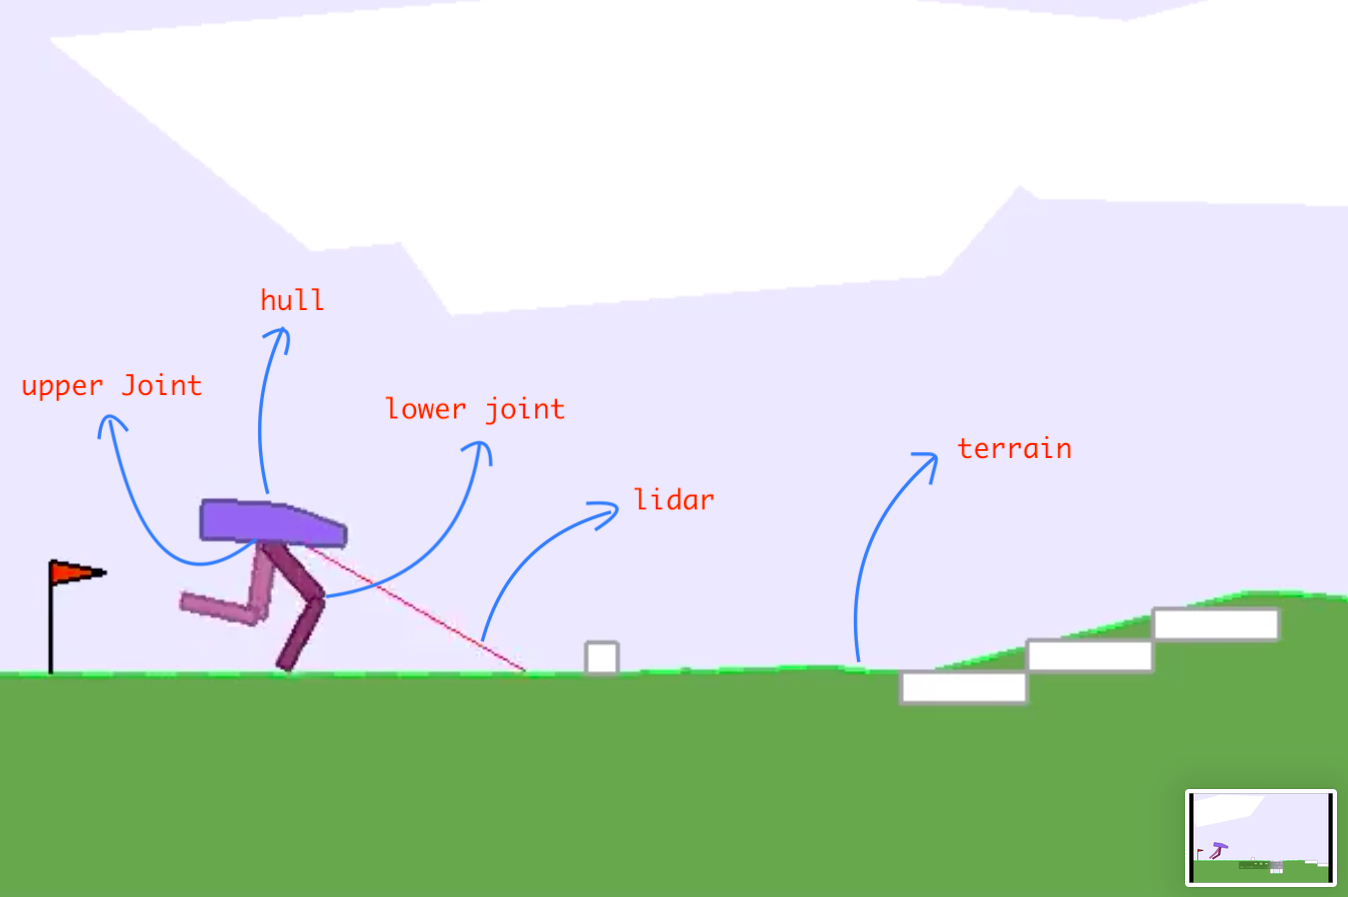
\includegraphics[width=150mm,height=75mm]{Pictures/bipedal.png}
\caption{Bipedal Walker Description [\cite{bipedalPic:2019}]}
\label{bipedal}
\end{figure}

Teach the bipedal robot to walk from starting to end without falling, thus maximizing the reward. Reward is given for moving forward, total 300+ points up to the far end. If the robot falls, it gets -100. Applying motor torque costs a small amount of points, hence more optimal agent will get better score. 

\section*{Algorithm}

\begin{figure}
\centering
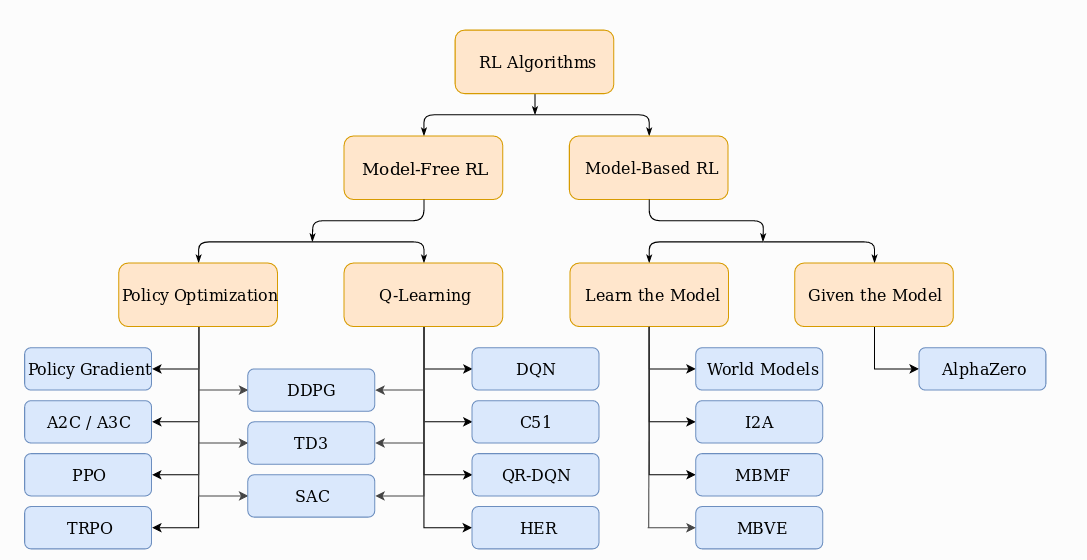
\includegraphics[width=150mm,height=75mm]{Pictures/RLAlgoChart.png}
\caption{A non-exhaustive, but useful taxonomy of algorithms in modern RL. [\cite{rlIntro2:2019}]}
\label{chart}
\end{figure}

\begin{itemize}
    \item {\bf Deterministic policy} maps state to action without uncertainty. It happens when you have a deterministic environment like a chess table. {\bf Stochastic policy} outputs a probability distribution over actions in a given state. 
    \item A {\bf model of the environment} means a function which predicts state transitions and rewards. {\bf Model-free RL} algorithms are those that make no effort to learn the underlying dynamics that govern how an agent interacts with the environment.
    \item {\bf Policy gradient} algorithms utilize a form of policy iteration: they evaluate the policy, and then follow the policy gradient to maximize performance.   
    \item In {\bf Q learning}, We constantly update a Q-Table, which is a lookup table where we calculate the maximum expected future rewards for action at each state. Basically, this table will guide us to the best action at each state.
    \item {\bf Off-policy} algorithms generally employ a separate behavior policy that is independent of the policy being improved upon; the behavior policy is used to simulate trajectories. A key benefit of this separation is that the behavior policy can operate by sampling all actions, whereas the estimation policy can be deterministic
    \item The {\bf TD error} signal is excellent at compounding the variance introduced by your bad predictions over time. It is highly suggested to use a replay buffer to store the experiences of the agent during training, and then randomly sample experiences to use for learning in order to break up the temporal correlations within different training episodes. This technique is known as experience replay.
    \item {\bf Actor-critic} combines the benefits of both approaches from policy-iteration method as PG and value-iteration method as Q-learning. The network will estimate both a value function V(s) (how good a certain state is to be in) and a policy $\pi$(s).
    \item The {\bf critic}’s output is simply the estimated Q-value of the current state and of the action given by the actor. The deterministic policy gradient theorem provides the update rule for the weights of the actor network. The critic network is updated from the gradients obtained from the TD error signal.
    \item DDPG is an actor-critic algorithm; it primarily uses two neural networks, one for the actor and one for the critic. These networks compute action predictions for the current state and generate a temporal-difference (TD) error signal each time step. The input of the actor network is the current state, and the output is a single real value representing an action chosen from a continuous action space.[\cite{ddpgTutorial:2019}]
\end{itemize}

\section* {Results and Analysis}

We got the following results:
\begin{itemize}
\item Initially tries different things and fails, getting bad rewards.
\item Learns that should not hit the ground.
\item Reward better but not enough, decides to move.
\item Cannot walk properly but still tries to not hit the ground.
\item Finally starts taking first steps.
\item The Final Training after 2000 episodes.
\item The accompanying graph shows that reward shows an increasing trend.
\end{itemize}

\includemedia[
width=1.1\linewidth,
height=1\linewidth,
activate=pageopen,
addresource=bipedal.mp4,
flashvars={source=bipedal.mp4}
]{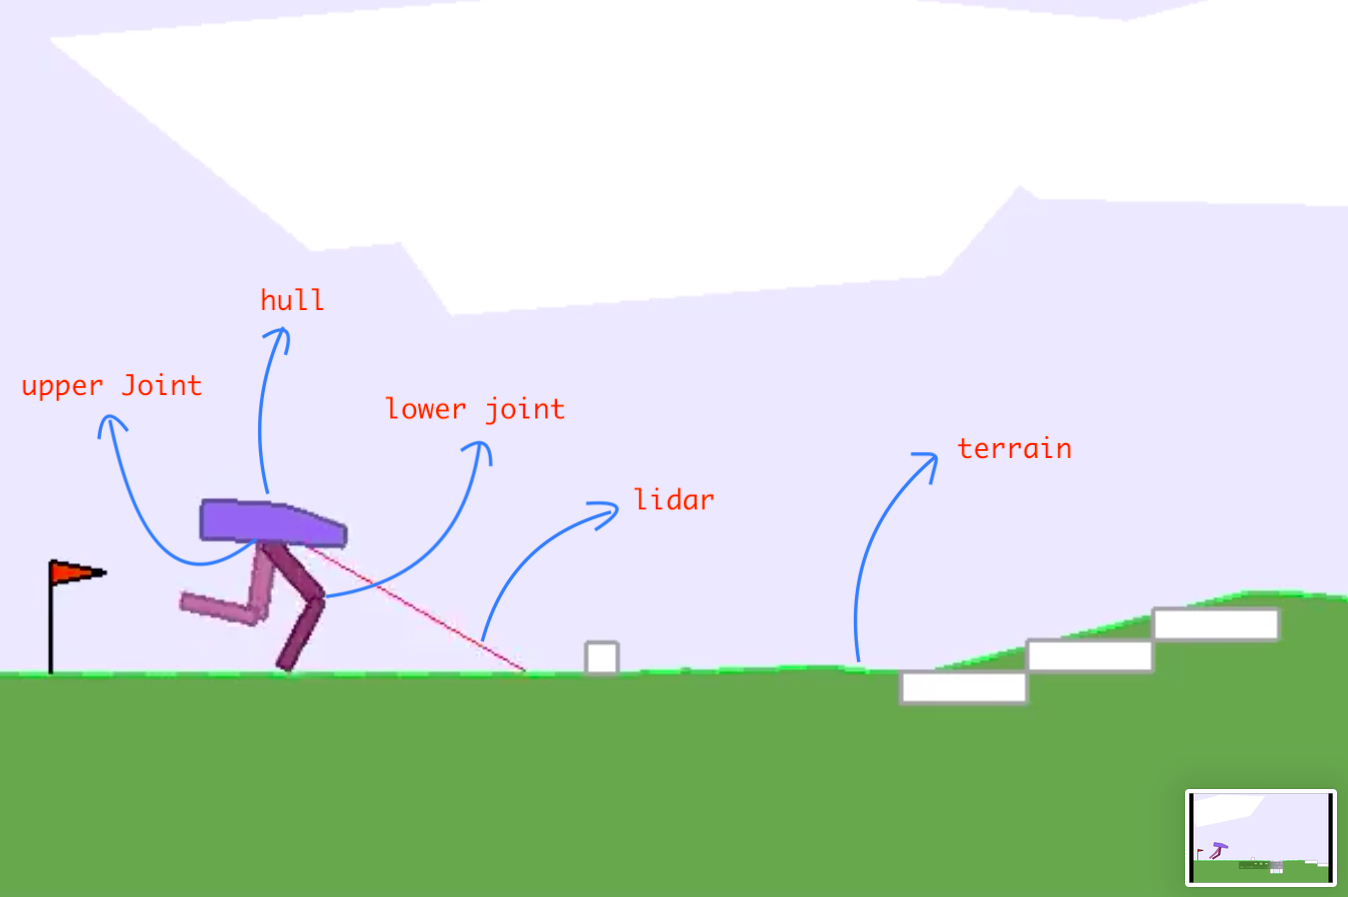
\includegraphics{Pictures/bipedal.png}}{VPlayer.swf}

\clearpage

\begin{figure}
\centering
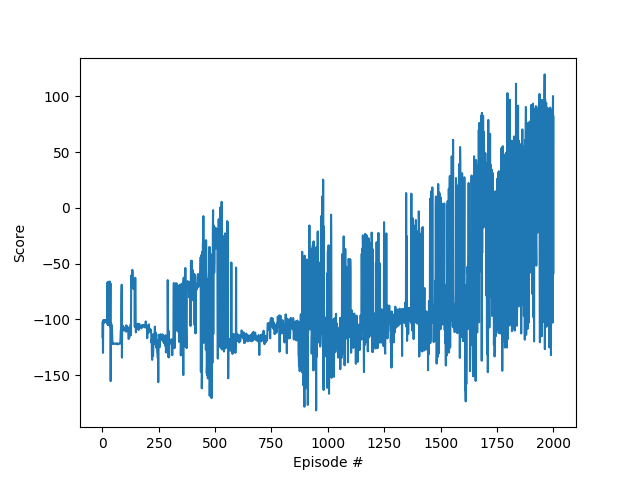
\includegraphics[scale=0.98]{Pictures/graph.png}
\caption{Rewards show an upward trend with increasing episodes}
\label{Frog}
\end{figure}

\section*{Conclusions}
Using Deep Deterministic Policy Gradient algorithm, it is possible to train a bipedal robot to walk. With just 2000 episodes of training(~3hrs) our agent learned to walk considerably well. Hence, this algorithms can be used to solve some real life problems such as teaching humanoid robots to walk without explicit programming.

\section*{Future Work}
The agent currently takes state input directly from gym environment, In the future we aim to take input directly from screen and use computer vision techniques to convert the input to the desired state. This would enable us to deploy the model in real world humanoid robots.

\clearpage

\bibliographystyle{apa}
\bibliography{Bibliography}


\end{document}